\documentclass[12pt, a4 paper]{article}
\usepackage[british]{babel}
\usepackage{graphicx, hyperref, xcolor, fancyhdr, amssymb, amsmath, amsthm, tikz, listings}
\usepackage[framemethod=TikZ]{mdframed}
\usepackage{mathrsfs}
\usepackage[acronym, toc]{glossaries}
\usepackage{pdfpages}
\usepackage{svg}
\usepackage{algorithmic}
\usepackage[ruled, linesnumbered]{algorithm2e}
\usepackage{pgfgantt, lscape}
\usepackage{fontawesome}

\usetikzlibrary {arrows.meta,automata,positioning} 
\usetikzlibrary{automata}

% Colors definition
\definecolor{isa_red}{RGB}{255, 58, 71}
\definecolor{isa_orange}{RGB}{219, 130, 57}
\definecolor{isa_light_blue}{RGB}{0, 163, 255}
\definecolor{isa_blue}{RGB}{0, 103, 158}
\definecolor{isa_dark_blue}{RGB}{26, 0, 253}
\definecolor{isa_green}{RGB}{0, 157, 97}
\definecolor{isa_dark_green}{RGB}{0,131, 0}
\definecolor{isa_purple}{RGB}{174, 5, 238}

% Define custom language for syntax highlighting
\lstdefinelanguage{Isabelle}{
  % List of custom keywords
  keywords=[1]{definition, if, then, else, let, in, case, of, do, SOME, lemma, note, THE},
  % Custom keyword styles
  keywordstyle=[1]\color{isa_blue},
  keywords=[2]{where, and},
  keywordstyle=[2]\color{isa_green},
  keywords=[3]{RETURNT, monadic_WHILEIET, SPEC, ASSERT, consume, cost},
  keywordstyle=[3]\color{isa_red},
  keywords=[4]{assume, define},
  keywordstyle=[4]\color{isa_light_blue},
  literate={`}{\textasciigrave\ }1,
  % Other language elements styles
  commentstyle=\color{isa_dark_green},
  string=[b]{''},
  stringstyle=\color{isa_purple},
  numberstyle=\tiny\color{isa_dark_blue},
  % Frame and background settings
  frame=l,
  framerule=3pt,
  rulecolor=\color{black!15},
  backgroundcolor=\color{black!5},
  % Other settings
  basicstyle=\ttfamily\small,
  breaklines=true,
  breakatwhitespace=true,
  showstringspaces=false,
  showtabs=false,
  tabsize=2
}
\lstset{%
  language=Isabelle,
  columns=fixed,
  extendedchars,
  basewidth={0.5em,0.45em},
  basicstyle=\ttfamily,
  mathescape=true
}

% editorial comments in the text or in marginal notes
% 1st argument: initials of the person making the comment,
% 2nd argument: comment to insert
\long\def\ednote#1#2{\par\noindent\framebox{\begin{minipage}{.98\linewidth}\linespread{.7}\footnotesize #1: #2\end{minipage}}\par}
\newcommand{\edmargin}[2]{\marginpar{\raggedright\linespread{.7}\tiny #1: #2}}

% redefine proof environment with grey background and black square at the end
\renewenvironment{proof}[1][Proof]{\begin{mdframed}[backgroundcolor=black!5, topline=false, rightline=false, bottomline=false, linecolor=black!15, linewidth=3pt]{\noindent\textit{#1.}\ }}{\noindent\par\hfill$\blacksquare$\end{mdframed}}

% \usepackage{times}

\hypersetup{
    colorlinks,
    linkcolor={red!60!black},
    citecolor={blue!80!black},
    urlcolor={blue!80!black}
}

% \pagestyle{fancy}
% \renewcommand\headrulewidth{.5pt}
% \fancyhead[L]{
%     V. Trélat
% }

% \fancyhead[C]{
%     \textbf{Verification in Isabelle/HOL of Hopcroft's algorithm for minimizing DFAs including runtime analysis}
% }

% \fancyhead[R]{
%     % Current section
%     \ifnum\c@secnumdepth>0
%         \thesection
% }

\newcommand{\midtilde}{\raisebox{0.5ex}{\texttildelow}}

\newcommand{\isavar}[1]{{\color{isa_dark_green}\text{#1}}}
\newcommand{\isafixed}[1]{{\color{isa_dark_blue}\text{#1}}}

% theorems
\theoremstyle{definition}
\newtheorem{theorem}{Theorem}
\newtheorem{lemma}{Lemma}
\newtheorem{remark}{Remark}
\newtheorem{definition}{Definition}
\newtheorem{requirement}{Requirement}

% Glossary

\makeglossaries

% \newacronym{tiaa}{TIAA}{This Is An Acronym}

\begin{document}

\begin{titlepage}
    \begin{center}
        \vfill
        
\includegraphics[height=1.5cm]{img/logoTUM.png}
        \hfill
        
\includegraphics[height=1.5cm]{img/logoartem.png}
        \hfill
        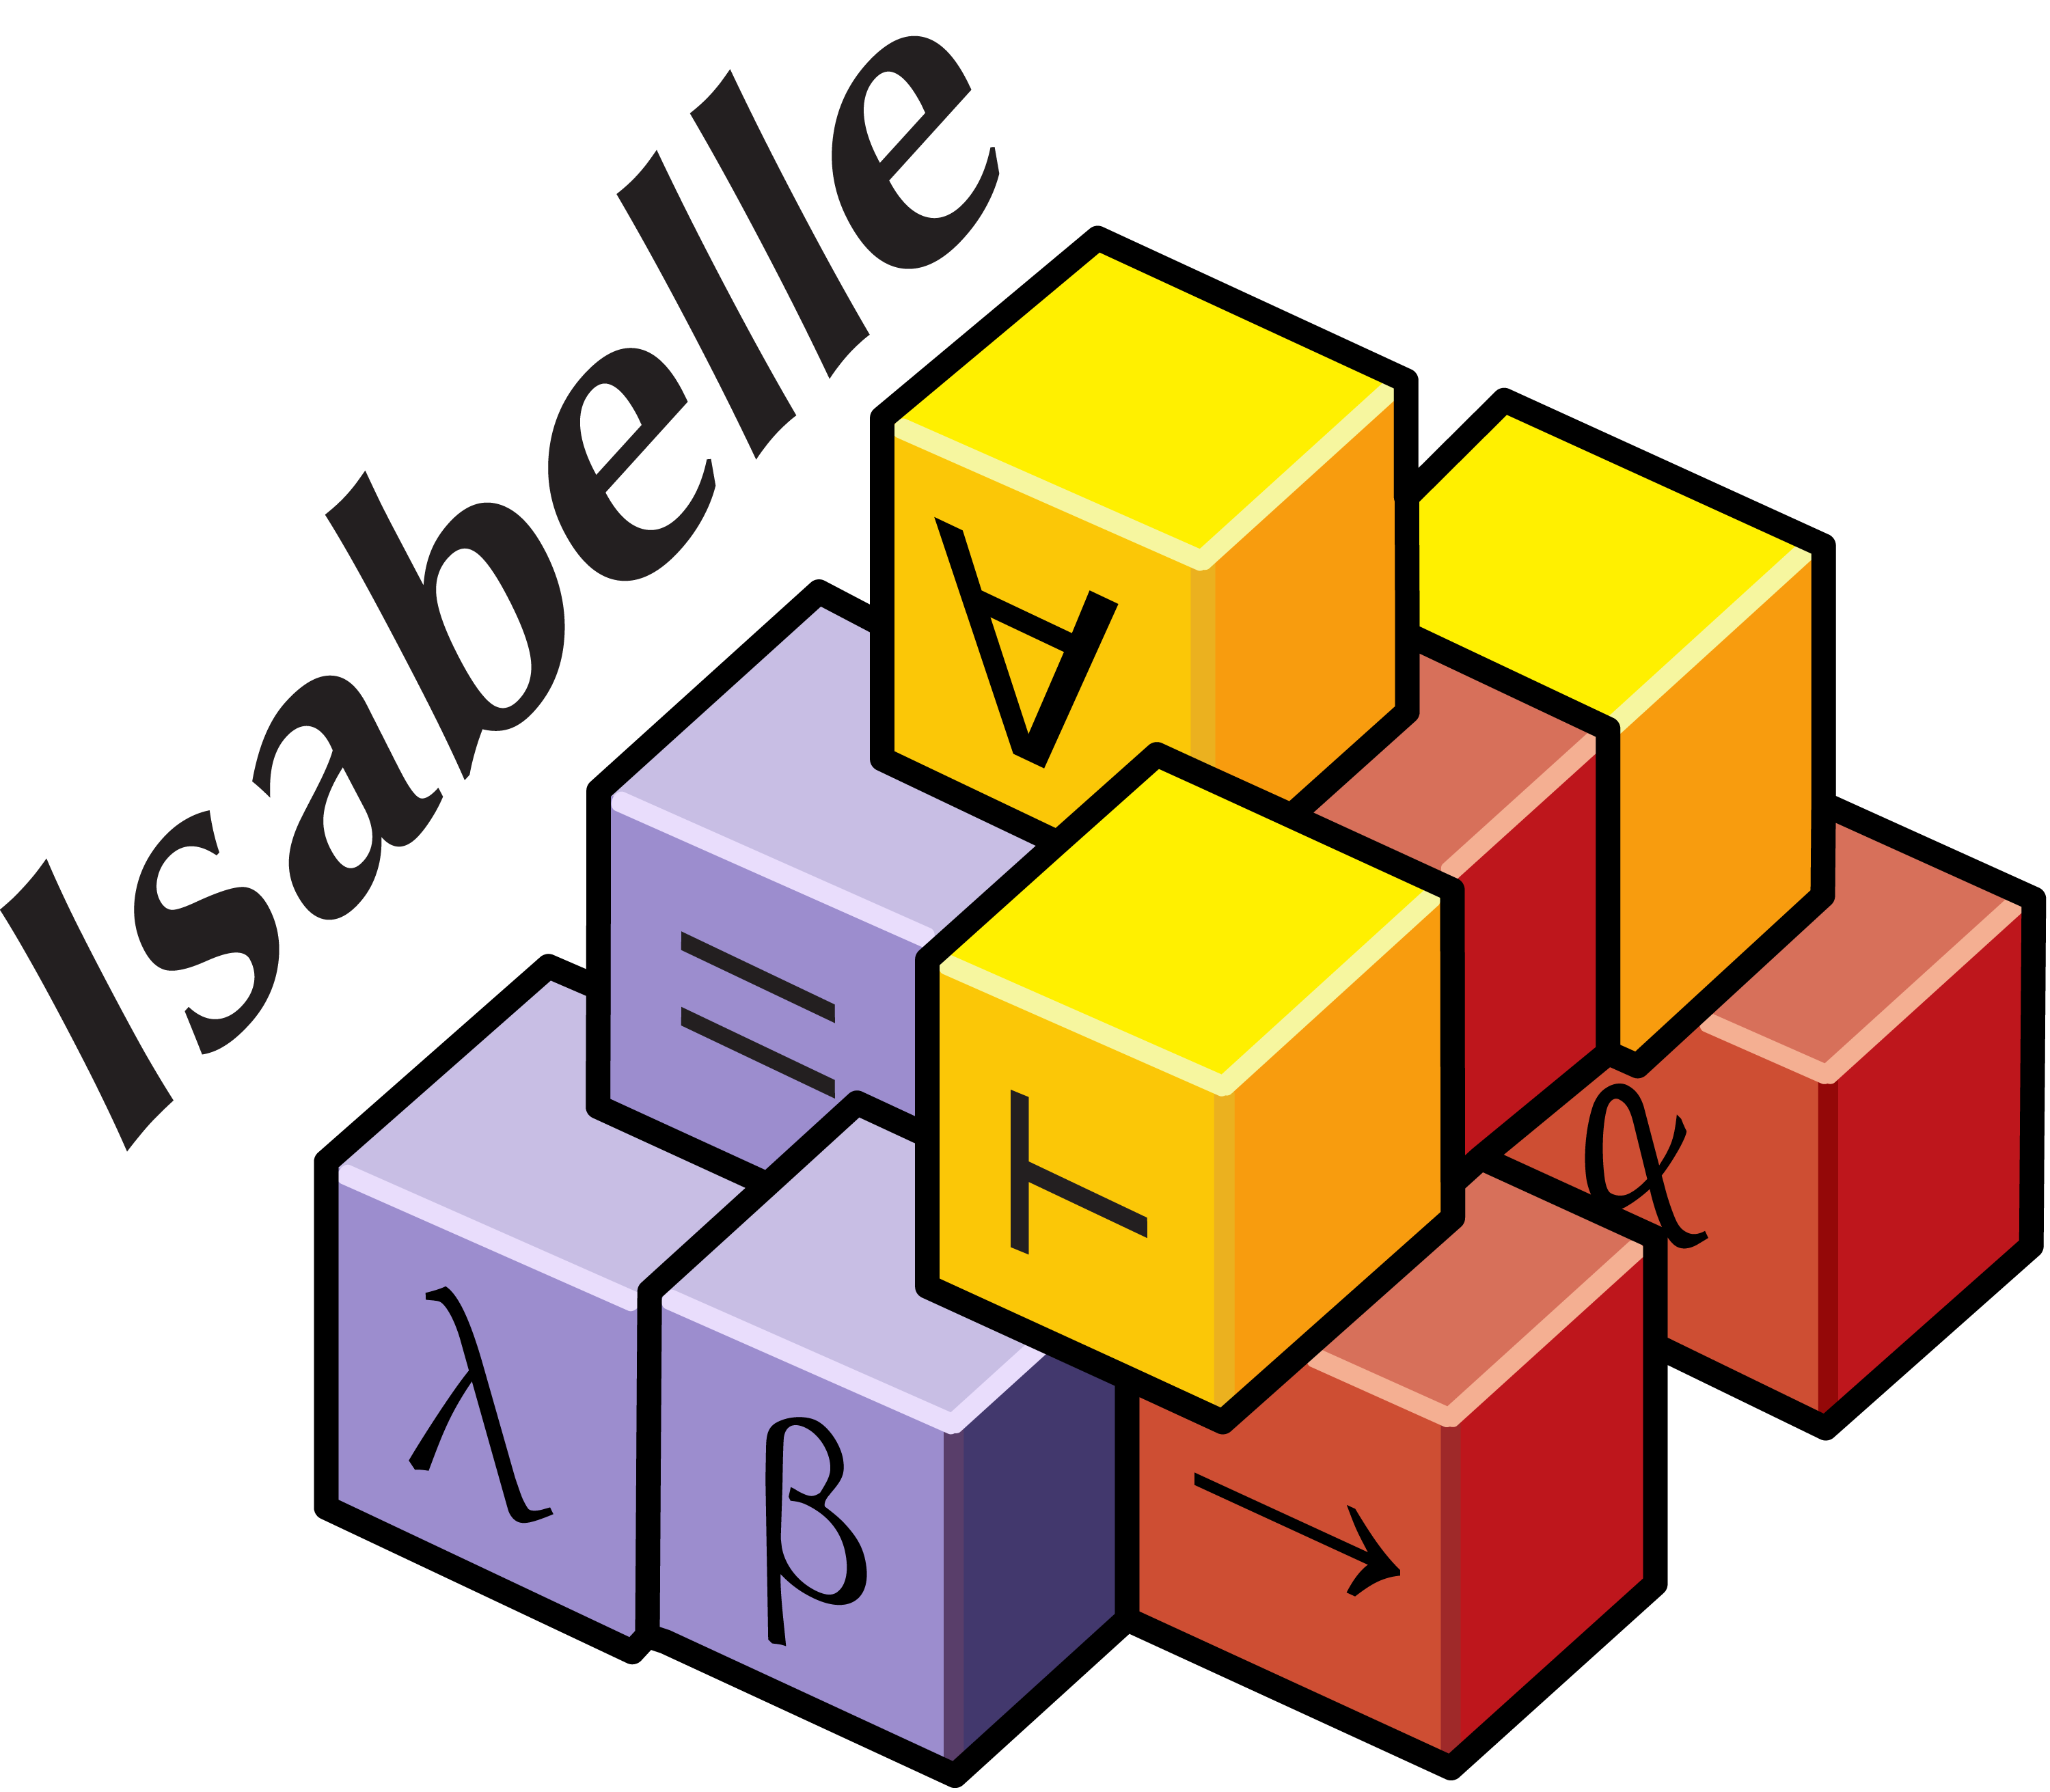
\includegraphics[height=1.5cm]{img/logoisabelle.png}
        \vfill
    \end{center}
    \begin{center}
        
        \textbf{Final year internship report}
        \vfill

        \large{\textbf{Verification in Isabelle/HOL of Hopcroft's algorithm for minimizing DFAs including runtime analysis}}
    \end{center}
    
    \vfill
    
    \begin{center}
        \textbf{Vincent Trélat}\\
        \vspace{1cm}
        \textit{\today}
    \end{center}
    \vfill
    \begin{center}
        
\includegraphics[height=1.2cm]{img/logoGE.png}
        \hfill
        
\includegraphics[height=1.2cm]{img/logoUL.png}
    \end{center}
\end{titlepage}

\tableofcontents

\pagebreak

\section{Preamble}

This report is the result of a 6-month internship at the Chair of Logic and Verification of the Technical University of Munich (TUM) under the supervision of \href{https://www21.in.tum.de/~nipkow/}{Tobias Nipkow} and \href{https://people.utwente.nl/p.lammich}{Peter Lammich}.

The main goal of this internship was to verify Hopcroft's algorithm for minimizing DFAs \cite{Hop71} in Isabelle/HOL and to analyze its worst-case time complexity using the Refinement Framework \cite{lammich:ref}.
Some considerable work had already been carried out by Peter Lammich and Thomas T\"urk on the proof of correctness ten years ago in an older version of Isabelle \cite{lammich:hop}.
The goal was to port this proof to the latest version of Isabelle and to extend it with a time complexity analysis using the NREST framework, namely the extension of the Refinement Framework to time \cite{refwithtime}.

In order to bring the reader closer to the reality of the project, some sections of this report dive a little deeper into the details of the interesting parts of my research. They are marked with the following gear symbol \faGears\ and can be skipped without loss of understanding of the main ideas.

\pagebreak

\section{Technical University of Munich}

The Technical University of Munich (TUM) stands as a beacon of academic excellence, renowned globally for its commitment to cutting-edge research, innovation, and education. Nestled in the heart of Germany, TUM's legacy spans over 150 years, consistently ranking among the top universities worldwide\footnote{TUM is ranked first in Europe in Computer Science and Mathematics. }. At TUM, scholars and students alike converge to explore and shape the forefront of various fields, fostering a dynamic environment that thrives on intellectual curiosity and collaboration.

Within the expansive landscape of TUM's academic endeavors lies the Chair of Logic and Verification -- a distinguished hub of expertise dedicated to the study and application of formal methods -- which operates at the intersection of computer science, mathematics, logic and engineering, harnessing the power of logical reasoning to ensure the precision and reliability of complex systems.

Among the illustrious figures leading the charge at the Chair of Logic and Verification is Professor Tobias Nipkow. A luminary in the realm of formal methods, he has made indelible contributions to the development and propagation of logical verification techniques.

Central to the Chair's accomplishments is the Isabelle proof assistant -- an innovation born from the ingenuity of Professor Tobias Nipkow and his dedicated team. Isabelle stands as a testament to the power of collaborative intellect, serving as a versatile tool for rigorous formal reasoning. This proof assistant facilitates the creation, manipulation, and verification of mathematical proofs, underpinning the very essence of formal methods' application. Its impact reverberates not only through academic corridors but also through the industries and systems that rely on robust verification.

In summary, the Technical University of Munich's Chair of Logic and Verification represents an ecosystem of brilliance, where researchers, developers, and applied experts converge to elevate the tenets of formal methods. Professor Tobias Nipkow's visionary leadership and the Isabelle proof assistant embody the spirit of innovation that defines this dynamic academic haven, propelling the boundaries of formal reasoning and verification.

\section{Introduction}

Since the whole project relies on many deeply theoretical notions such as abstraction, logic or semantics, this section only gives a brief introduction to formal methods in general and their purpose.

\bigskip

Formal methods refer to a field of theoretical computer science whose main purpose is to provide logical links between mathematics and programming languages, so that one can state logical properties about formally described algorithms or mathematical procedures and relate them to actual implementations.
The main application of formal methods is to prove correctness of programs with respect to a specification, i.e.\ a set of rules which must hold throughout the execution of the program.
Such a program is then ensured to behave in a way\footnote{In the context of industrial applications, we often differentiate between two sorts of assertions, namely safety properties and liveness properties, so that we can explicitly check that the system works (it is ``alive'') and that it is safe (it works properly).} that is intended by its specification.

Such work is usually carried out using a proving assistant such as \href{https://isabelle.in.tum.de}{Isabelle}, i.e.\ a program with an implemented logic allowing to reason with respect to that logic.
Isabelle has the advantage to relie on a really light kernel, which is the only part that can only be trusted. Everything else -- i.e. librairies, called theories -- stems from this kernel.
It also has nice interface with \LaTeX syntax adding little overhead to usual mathematical notations and is very flexible in terms of syntax and semantics.

A common way to proceed when we want to prove correctness of an algorithm and generate correct executable code is to follow a top-down strategy via successive refinements.
We start from the highest level -- i.e.\ with the highest level of abstraction -- and we refine towards the implementation.
As an example, if an algorithm manipulates sets at the abstract level, we may use lists or trees in its implementation.
When performing a refinement, we have to give links -- and prove them -- between levels, e.g. that the behavior of the refined one does not contradict the abstract one.
In Peter Lammich's Refinement Framework \cite{lammich:ref}, this is done via binary relations and abstraction/concretization functions\footnote{A concretization function maps an abstract value to a set of concrete values and conversely for an abstraction function, so that invariants can be carried and preserved through the refinements.
For example, we may abstract the set $\mathbb{Z}$ of integers to $\{Neg, Zero, Pos\}$ where $Pos$ (resp.\ $Neg$) represents positive (resp.\ negative) integers and $Zero$ represents the singular set $\{0\}$.}. The Refinement Framework is briefly introduced in the next section.

\bigskip

If formal methods allow for correctness and termination theorems, it is less trivial to analyze complexity of a program, e.g.\ in terms of time or memory consumption.
Since complexity of a program is not a logical property, but a property of the execution of the program, a model of computation must be defined, i.e.\ a way to execute the program, and then prove that the execution of the program in this model is equivalent to the execution of the program in the real world.
Maximilian Haslbeck and Peter Lammich have extended the Refinement Framework to include worst-case time complexity analysis in Isabelle \cite{refwithtime} and have also implemented a verified framework to analyze algorithms down to LLVM code \cite{fewdollarsmore}.
The principle is to model costs of operations with resources and currencies and embed this new dimension in the program, where operations consume resources.

\bigskip

Since the project also relies on automata theory, it is recommended to have some basic knowledge about automata theory and formal languages.

\subsection{The Refinement Framework}

The Refinement Framework \cite{lammich:ref} is a methodology for designing and verifying computer systems, particularly in critical applications like aviation and healthcare.
It was mostly developed by \href{https://people.utwente.nl/p.lammich}{Peter Lammich} and \href{https://www21.in.tum.de/~haslbema/}{Maximilian P. L. Haslbeck}, often in collaboration with tools like Isabelle.

At its core, the Refinement Framework provides a systematic way to start with a high-level, abstract description of a system and gradually refine it into a concrete implementation.
It works the same way one would build a house. First, a basic blueprint with the overall design and room layouts is designed: it is the abstract specification. Then, this plan is gradually refined by adding more detail at each step. For instance, the materials, dimensions, and exact placement of walls, plumbing, and electrical systems might be specified. Each refinement step brings the model closer to the actual construction until a fully detailed plan is obtained and ready for builders to follow.

Software development, is completely analogous. We start with a high-level description of what a software system should do (the abstract specification), and it is refined through several stages, adding more and more detail until we have a concrete and reliable software implementation. This process helps ensure that the final software system matches what one originally intended, and it provides a way to verify that it works correctly.

The key benefit of the Refinement Framework is that it helps catch errors and problems early in the development process, reducing costly mistakes and improving the quality of the final product. It's a systematic way to bridge the gap between abstract concepts and real-world software, making sure they align properly.

\subsection{Setting up the environment \faGears}
In order to be able to comfortably browse the theories and inspect the proofs, it is recommended to use Isabelle\footnote{The project was carried out using \href{https://isabelle.in.tum.de/}{Isabelle2022}.}/jEdit. Yet, the project is not part of the \href{https://www.isa-afp.org/}{Archive of Formal Proofs} (AFP) and can only be downloaded from the \href{https://github.com/VTrelat/Hopcroft_Verif}{GitHub repository}.

Then, building an image of the main framework is strongly recommended, as it will greatly speed up the compilation of the theories, especially for the time complexity analysis. This may take a few minutes, but only needs to be done once:
\begin{lstlisting}[language=bash]
cd Hopcroft_Verif/Hopcroft_Time
isabelle build -d . -l Isabelle_LLVM_Time Hopcroft_Time.thy
\end{lstlisting}

Isabelle may then be launched with jEdit by running the following command. This will open the main theory file \texttt{Hopcroft\_Time.thy} in jEdit and should take less than a minute:
\begin{lstlisting}[language=bash]
isabelle jedit -d . -l Isabelle_LLVM_Time Hopcroft_Time.thy
\end{lstlisting}

\subsection{Hopcroft's algorithm}
John E. Hopcroft's algorithm for minimizing deterministic finite automata (DFA) was first presented in his original 1971 paper \cite{Hop71} as a formal algorithm.
It has been a major breakthrough in the field of automata theory, since it allowed for minimization in linearithmic\footnote{$O(n \log n)$} time in the worst case\footnote{Other minimization algorithms were presented prior to Hopcroft, e.g.\ by Moore (quadratic) or Brzozowski (exponential).}.
Thanks to this, minimization has become almost costless and thus this algorithm has been widely used in the field of formal verification, e.g.\ in model checking, since it allows to reduce the size of the automaton to be verified.

The formal idea behind the algorithm is to partition the set of states of the DFA into equivalence classes, i.e.\ sets of states that are equivalent\footnote{Two states are equivalent if they accept the same language.} with respect to the language they recognize.
The algorithm starts with two partitions, namely the set of final states and the set of non-final states.
Then, it iteratively refines the partitions by splitting them into smaller ones until no more refinement is possible.
The algorithm is guaranteed to terminate since the number of partitions is finite and strictly decreases at each iteration.
The equivalence class of the set of states of the DFA is then the set of partitions, so that any two different sets of states from that partition recognize different languages.

\subsection{Original formalization \faGears}

\begin{algorithm}[H]
\SetAlgoLined
\caption{Hopcroft's original formal algorithm}
\label{alg:original}
\KwData{a finite DFA $\mathcal{A} = (\mathcal{Q}, \Sigma, \delta, q_0, \mathcal{F})$}
\KwResult{the equivalence class of $\mathcal{Q}$ under state equivalence}
Construct $\delta^{-1}(q, a) := \{t \in \mathcal{Q}\ |\ \delta(t, a) = q\}$ for all $q \in \mathcal{Q}$ and $a \in \Sigma$ \;\label{alg:original:1}
Construct $P_1 := \mathcal{F}$, $P_2 := \mathcal{Q} \setminus \mathcal{F}$ and $s_{a,i} := \{q \in P_i \ | \ \delta^{-1}(q, a) \neq \varnothing \}$ for all $i \in \{1, 2\}$ and $a \in \Sigma$ \;
Let $k := 3$ \;
For all $a \in \Sigma$, construct $L_a := \underset{1 \leq i < k}{\operatorname*{arg\,min}}\ \left| s_{a, i} \right|$ \; \label{alg:original:4}
\While{$\exists a \in \Sigma, L_a \neq \varnothing$\label{alg:original:loop}}{
    Pick $a \in \Sigma$ such that $L_a \neq \varnothing$ and $i \in L_a$ \; \label{alg:original:pick}
    $L_a := L_a \setminus \{i\}$ \;
    \ForAll{$j < k, \exists q \in P_j, \delta(q, a) \in s_{a,i}$}{
        $P'_j := \{t \in P_j\ |\ \delta(t, a) \in s_{a,i} \}$ and $P''_j := P_j \setminus P'_j$ \;
        $P_j := P'_j$ and $P_{k} := P''_j$; construct $s_{a,j}$ and $s_{a,k}$ for all $a \in \Sigma$ accordingly \;
        For all $a \in \Sigma$, $L_a := \begin{cases}
        L_a \cup \{j\} & \text{if $j \notin L_a \land \left| s_{a,j} \right| \leq \left| s_{a,k} \right|$} \\
        L_a \cup \{k\} & \text{otherwise}
        \end{cases}$ \;
        $k := k + 1$ \;
    }
}
\end{algorithm}

\bigskip

Algorithm~\ref{alg:original} is a direct translation of the original algorithm from \cite{Hop71} with only slight changes in the notations.

\subsection{Modern formalization}

The algorithm is now usually given in a more mathematical and formalised way\footnote{See for example \cite{esparza2023automata}.}, which loosens up the choice for an implementation.
The algorithm is given below in Algorithm~\ref{alg:modern} using sets and partitions.


\begin{algorithm}[H]
    \SetAlgoLined
    \caption{Hopcroft's algorithm in a modern style}
    \label{alg:modern}
    \KwData{a finite DFA $\mathcal{A} = (\mathcal{Q}, \Sigma, \delta, q_0, \mathcal{F})$}
    \KwResult{the language partition $P_\ell$}
    \eIf{$\mathcal{F} = \varnothing \lor \mathcal{Q} \setminus \mathcal{F} = \varnothing$}{
        \Return $\mathcal{Q}$
    }{
        $\mathcal{P} := \{ \mathcal{F}, \mathcal{Q} \setminus \mathcal{F} \}$ \;
        $\mathcal{W} := \{ (a, \min \{ \mathcal{F}, \mathcal{Q} \setminus \mathcal{F}\}), a \in \Sigma \}$ \;
        \While{$\mathcal{W} \neq \varnothing$}{
            Pick $(a, C)$ from $\mathcal{W}$ and remove it\;
            \ForAll{$B \in \mathcal{P}$}{
                Split $B$ with $(a, C)$ into $B_0$ and $B_1$ \;
                $\mathcal{P} := (\mathcal{P} \setminus \{B\}) \cup \{B_0, B_1\}$ \;
                \ForAll{$b \in \Sigma$}{
                    \eIf{$(b, B) \in \mathcal{W}$}{
                        $\mathcal{W} := (\mathcal{W} \setminus \{(b, B)\}) \cup \{(b, B_0), (b, B_1)\}$ \;
                    }{
                        $\mathcal{W} := \mathcal{W} \cup \{(b, \min \{ B_0, B_1 \})\}$ \;
                    }
                }
            }
        }
    }
\end{algorithm}

\bigskip

We justify this transformation.
First, instead of storing indices for the blocks, we directly deal with sets and explicitly work with a partition $\mathcal{P}$ of $\mathcal{Q}$.
Then, we define splitters.

\begin{definition}
    Let $\mathcal{A} = (Q, \Sigma, \delta, q_0, I, F)$ be a DFA. Let $P$ be a partition of $Q$. Let $B \in P$. For $a \in \Sigma$ and $C \in P$ we say that
    $(a, C)$ splits $B$ or is a splitter of $B$ if $$\exists q_1, q_2 \in B \quad \delta(q_1, a) \in C \land \delta(q_2, a) \notin C.$$
\end{definition}
\begin{remark}
    If $(a, C)$ is a splitter of $B$, $P$ can be updated to $P \setminus \{B\} \cup \{B', B''\}$, where $$B' := \{q \in B \ | \ \delta(q, a) \in C\} \text{ and } B'' := B \setminus B'.$$
\end{remark}

\begin{definition}
    For a splitter $s \in \Sigma \times P$, we define its size $\| s \|$ as the size of its second component, i.e.\ if $s = (a, C)$, then $\| s \| := |C|$.
\end{definition}


In Algorithm \ref{alg:original}, picking an index $i \in L_a$ corresponds to picking a set $s_{a, i}$, i.e.\ -- by definition -- the subset of $P_i$ of states having at least one predecessor.
We cannot directly replace $L_a$ and $s_{a, i}$ by a set of splitters $(a, P_i)$ as is, however the next step in the algorithm is to go over all blocks in the partition that have a successor in $s_{a, i}$.
If such a block $B$ is found, it is split into two blocks, namely the set of states having a successor in $s_{a, i}$ and the others.
Overall, we look for $B$ such that $P_i$ has a predecessor in $B$. We add the condition that $B$ must also have at least one successor not in $P_i$ to avoid splitting $B$ into $\{B, \varnothing\}$.
Since this is equivalent to splitting $B$ with $(a, P_i)$, we can replace $L_a$ by a set of splitters $(a, P_i)$.
Since the symbol $a$ is chosen such that $L_a \neq \varnothing$, we can define a workset $\mathcal{W}$ of all splitters, with all symbols of $\Sigma$. Therefore, $L_a$ is empty if and only if there is no $a$-splitter in $\mathcal{W}$.
Because testing emptiness is equivalent to testing membership, and because of the existential quantifier in the definition of splitters, the $s_{a, i}$ are no longer needed.

We can explicitly write the trivial cases where either $\mathcal{F}$ or $\mathcal{Q}\setminus\mathcal{F}$ is empty to improve performance for this specific case.
This is not done in Algorithm \ref{alg:original} but this does not produce wrong results.
If one of the two sets is empty, one of the $s_{a, 1}$ or $s_{a, 2}$ will be empty for all $a \in \Sigma$, and the \textit{while} loop will be entered $|\Sigma|$ times but the inner \textit{for} loop will never be entered.
This results in a useless $O(|\Sigma|)$ computation.
Another difference in that case is that it would return the partition $\min\{\mathcal{F}, \mathcal{Q}\setminus\mathcal{F}\}$ -- where $\min$ returns the set with the least number of elements --  which we avoid in the modern version by just returning $\mathcal{Q}$.

\section{Overview of the project}

\subsection{Objectives of the project}

The project can be divided into two main parts:
\begin{itemize}
    \item[(i)] porting the old formalization of the algorithm and its proof of correctness to the latest version of Isabelle,
    \item[(ii)] extending the proof with a time complexity analysis using the NREST Framework \cite{refwithtime}, i.e.\ the extension of the Refinement Framework to time.
\end{itemize}

The first part is rather straightforward since it only involves a good understanding of the original proof and the Refinement Framework. The main proofs are fixed by finding syntax changes and adapting them accordingly.

the second one is more challenging since it requires a good understanding of the algorithm and the Refinement Framework, as well as a good knowledge of the NREST Framework.


\begin{landscape}
\subsection{Gantt chart}
\begin{ganttchart}[
    hgrid,
    vgrid={*3{black,dotted}, *1{black, dashed}},
    x unit=0.59cm,
    y unit title=0.5cm,
    y unit chart=0.7cm,
    title height=1,
    title/.style={fill=gray!20},
    title label font=\bfseries,
    group/.append style={fill=green!20!black!70},
    bar/.style={fill=green!35!black!50},
    bar height=0.5,
    progress label text={\pgfmathprintnumber[precision=0,verbatim]{#1}\%},
    group left shift=0,
    group right shift=0
  ]{1}{24}

  % Months every 4 units
  \gantttitle{Gantt chart}{24} \\
  \gantttitle{March}{4}
  \gantttitle{April}{4}
  \gantttitle{May}{4}
  \gantttitle{June}{4}
  \gantttitle{July}{4}
  \gantttitle{August}{4}\\
  
  \ganttgroup{Porting old theories}{1}{5} \\
  \ganttbar{Reading documentation}{1}{2} \\
  \ganttbar{Fixing proofs}{2}{5} \\ \ganttnewline
  
  \ganttgroup{Time Complexity Analysis}{6}{22} \\
  \ganttbar{Paper proof}{6}{12} \\
  \ganttbar{Getting used to NREST}{9}{13} \\
  \ganttbar{Isabelle formalization}{13}{21} \\
  \ganttbar[bar/.append style={fill=orange!60}]{Proof of \texttt{estimate2\_decrease}}{14}{18} \\
  \ganttbar{Writing documentation}{20}{22}
\end{ganttchart}
\end{landscape}

\subsection{Main difficulties}

Like any project in formal methods, the main difficulty is to find a good abstraction level for the formalization and a good formalization. Fortunately, I could base mine on the existing one used for the proof of correctness in which the different levels of abstraction -- i.e.\ the different stages of refinement -- were already designed down to the implementation, so the choice for the datastructures was even already done.

Of course, paper proofs serve as foundations for the formal proof. I consider them as the ``fun'' part since paper is the first place where actual research starts. Draft proofs may also be considered as the ``easy'' part since a lot of details -- of implementation, or formal details -- are often omitted\footnote{Be it deliberate or not!} during this phase. Finding a good paper proof involves being cautious with potential inaccuracies that would make the formal proof harder at a later stage: it happens that a paper proof seems correct at first but is actually wrong or unprovable formally -- at least modulo some changes.

The ``real'' challenges lie in formalizing the different levels of abstraction: they should be gradual enough to make proofs digestible. My formalization follows the formalization used for the proof of correctness with slight adjustments for the time complexity analysis, so all the trouble I had with the formalization was linked to using the NREST framework properly. It involve theoretical notions of semantics and concepts such as, resources, currencies, and the NREST monad, but also practical notions such as specific commands or tactics in Isabelle that come with the framework.


\section{Proof of correctness}

Since the proof of correctness is not the purpose of this project, I just sketch the main ideas that are also helpful for the time complexity analysis and stand as a good introduction to the formalization.
John E. Hopcroft's original paper \cite{Hop71} contains a proof of correctness for his low-level algorithm, however the ideas behind the invariants are the same for the formalization.
The proof typically involves two main components: partition refinement and equivalence checking.

The basic idea of the proof is to show that the algorithm correctly partitions the states of the input DFA into equivalence classes, where states within the same class are indistinguishable from each other with respect to the language recognized by the DFA. This partition represents the minimal DFA that recognizes the same language as the input DFA.

The algorithm starts with an initial partition that distinguishes accepting states from non-accepting states. Then, it iteratively refines this partition by considering pairs of states that are currently in different equivalence classes and determining if they can be distinguished by a symbol from the input alphabet.

During each iteration, the algorithm examines each symbol in the alphabet and checks if it distinguishes any pair of states in different equivalence classes. If a symbol does distinguish a pair, it splits the equivalence class containing those states into two new classes. This process continues until no more splits can be made, and the resulting partition represents the minimal DFA.

To prove the correctness of Hopcroft's algorithm, one needs to show two key properties:
\begin{itemize}
    \item the resulting partition is a valid equivalence relation, meaning it satisfies the properties of reflexivity, symmetry, and transitivity,
    \item the resulting partition is indeed the minimal partition that correctly distinguishes states based on their language equivalence.
\end{itemize}

The proof typically involves reasoning about the behavior of the algorithm during each iteration, considering how the partition is refined inductively and ensuring that it converges to the minimal partition.

In the Refinement Framework, the algorithm is first described at the abstract level, so its correctness can be proved independently of any implementation details. Then, the algorithm is progressively refined into a concrete implementation, and the correctness of each refinement until the implementation is proved by showing that it refines the abstract algorithm.


\section{Time complexity analysis}

\subsection{Introduction}

In order to give a glimpse of my contributions to this project, this section sketches the main ideas behind the time complexity analysis of Hopcroft's algorithm, since it was the main goal of this internship. First, I give my raw notes on the paper proof. This acts as a pre-strucutred draft for the formalization in Isabelle. Then, I give a brief overview of the formalization in Isabelle.

\bigskip

The idea of the proof is the following: the algorithm can be reduced to a loop, so first, we find an upper bound\footnote{This upper bound will depend on some parameters such as an input (a letter) and a set of states of the automaton (a block of the partition).} for the time taken for an iteration of this loop. Then, we have to find how many iterations are executed until termination of the algorithm. To do so, we design what is referred to as an ``estimate'' of the time spent in the loop until its termination. At each step, this estimate is refined with the actual time taken by the previous steps, so that it decreases at each step. Finding a good estimate is the meat of the proof.

\subsection{Paper proof}

In a first time, we focus on the original algorithm presented in Algorithm~\ref{alg:original} in order to work on the arguments given in \cite{Hop71}.
The data structures used at that time were mostly linked lists, but let us rather give some requirements for the data structures instead of actual implementations.
The goal is to show that the algorithm can be executed in $O(m \cdot n \log n)$ time, where $m$ is the number of symbols in the alphabet and $n$ is the number of states in the DFA.

The following requirements come directly from \cite{Hop71} and are specific to the algorithm presented in Algorithm~\ref{alg:original}.

\begin{requirement}
    \label{req:1}
Sets such as $\delta^{-1}(q, a)$ and $L_a$ must be represented in a way that allows $O(1)$ time for addition and deletion in ``front position''\footnote{This does not make sense for sets and is specific for a data structure. What is meant here is a bit informal and designates a position directly accessible, e.g.\ the head for a stack, the value of the root for a tree, etc.}.
\end{requirement}

\begin{requirement}
    \label{req:2}
Vectors must be maintained to indicate whether a state is in a given set.
\end{requirement}

\begin{requirement}
    \label{req:3}
Sets such as $P_i$ must be represented in a way that allows $O(1)$ time for addition and deletion at any given position.
\end{requirement}

\begin{remark}
    \label{req:4}
From Req.\ \ref{req:2} and Req.\ \ref{req:3}, we can show that for a state $q$ in the representation of a set $P_i$ or $s_{a,i}$, its ``position'' -- in the implemented data structure -- must be determined in $O(1)$ time.
\end{remark}

\bigskip

\begin{lemma}
    In Algorithm \ref{alg:original}, lines \ref{alg:original:1} to \ref{alg:original:4} can be executed in $O(\left| \Sigma \right| \cdot \left| \mathcal{Q} \right|)$ time.
\end{lemma}
\begin{proof}
    The non trivial part is the computation of the inverse transition function $\delta^{-1}(q, a)$, for all $q \in \mathcal{Q}$ and $a \in \Sigma$. This can be done in $O(\left| \Sigma \right| \cdot \left| \mathcal{Q} \right|)$ time by iterating over $\Sigma$ and traversing the automaton (e.g.\ with a DFS) while keeping track of the predecessor at each step.
\end{proof}

\bigskip

\begin{lemma}\label{lem:time_iteration}
    An iteration of the \textit{while} loop in both algorithms for a splitter $s = (a, C)$ takes a time proportional to the number of transitions terminating in $C$ and the number of symbols in the alphabet, i.e. $\Theta\left(\left| \Sigma \right| \cdot \left| \delta^{-1}(C, a) \right| \right)$ time.
\end{lemma}
\begin{proof}
    We start by showing it for Algorithm \ref{alg:original}. We pick $a \in \Sigma$ such that $L_a \neq \varnothing$ and an $i \in L_a$. We need to examine all $j < k$ such that $\exists q \in P_j, \delta(q, a) \in s_{a,i}$ to construct the sets corresponding to splitting the block $P_j$ w.r.t.\ $a$ and $P_i$.

    Let $j < k$. From the definition of $s_{a,i}$, we obtain the following:
    \begin{align*}
        \exists q \in P_j, \delta(q, a) \in s_{a,i} &\iff \exists q \in P_j, \delta(q, a) \in P_i \land \underset{\text{true}}{\underbrace{\delta^{-1}(\delta(q, a), a) \neq \varnothing}} \\
        & \iff \exists q \in P_j, \delta(q, a) \in P_i
    \end{align*}
    Which corresponds to finding states in $P_j$ having an outgoing $a$-transition to a state in $P_i$, as represented in the following scheme:
    \begin{center}
        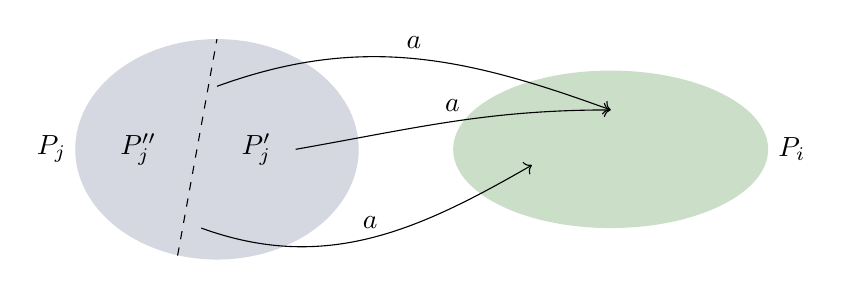
\begin{tikzpicture}
            \definecolor{color1}{RGB}{213, 216, 224}
            \definecolor{color2}{RGB}{202, 222, 200}
            
            \fill[color=color1] (0,0) ellipse (1.8cm and 1.4cm);
            \draw[dashed] (-0.5,-1.35) -- (0,1.4);
            \fill[color=color2] (5,0) ellipse (2cm and 1cm);
            
            \node at (-2.1,0) {$P_j$};
            \node at (-1,0) {$P''_j$};
            \node at (0.5,0) {$P'_j$};
            \node at (7.3,0) {$P_i$};

            \draw[->] (0, 0.8) to[in=160, out=20] node[above]{$a$} (5,0.5);
            \draw[->] (1,0) to[in=180, out=10] node[above]{$a$} (5,0.5);
            \draw[->] (-.2,-1) to[in=210, out=-20] node[above]{$a$} (4,-.2);
        \end{tikzpicture}
    \end{center}
    This set of states can be expressed via the inverse transition function:
    $$ \{q \in P_j\ |\ \delta(q,a) \in P_i \} = \left( \bigcup_{q' \in P_i} \delta^{-1}(q', a)\right) \cap P_j $$
    Since $\delta^{-1}$ was already computed in the first step of the algorithm, we can determine using req.\ \ref{req:3} whether a state of $\bigcup_{q \in P_i} \delta^{-1}(q, a)$ is also in $P_j$ in $\Theta(1)$ time.
    
    Thus, instead of examining $P_j$ for all $j < k$, we rather go through the table of $\delta^{-1}$ and for each state $q$ such that $\delta(q, a) \in P_i$, we know from req.\ \ref{req:4} that we can determine the index $j < k$ (because there are $k$ blocks) of the block $P_j$ containing $q$ in $\Theta(1)$ time.
    The sets $P'_j$ and $P''_j = P_k$ resulting from the partition can be constructed on the fly without any additional time cost. The construction of the sets $s_{b, j}$ and $s_{b, k}$ as well as the update of $L_b$ for all $b \in \Sigma$ can also be done on the fly but require $\Theta(1)$ time for each symbol $b \in \Sigma$ and thus add up to a total of $\Theta(\left| \Sigma \right|)$ time.
    %\ednote{VT}{the on-the-fly computation part is a little hand-waving...}

    Overall, one iteration of the loop runs in time
    $$\Theta \left( \left| \Sigma \right| \cdot \left| \bigcup_{q \in P_i} \delta^{-1}(q, a) \right| \right) $$

    \bigskip
    We now show the result for Algorithm \ref{alg:modern}. A splitter ${s =: (a, C)}$ is picked from $\mathcal{W}$.
    Then, we iterate over all blocks $B \in \mathcal{P}$ that may be split with $s$. Let $B \in \mathcal{P}$.
    \begin{align*}
        s\ \text{splits}\ B &\iff \exists q_1, q_2 \in B \quad \delta(q_1, a) \in C \land \delta(q_2, a) \notin C\\
        &\iff \{q_1 \in B, \delta(q_1, a) \in C\} \neq \varnothing \land \{q_2 \in B, \delta(q_2, a) \notin C\} \neq \varnothing \\
        &\iff \left(\bigcup_{q \in C} \delta^{-1}(q, a)\right)\cap B \neq \varnothing \land \left(\bigcup_{q \in B}\delta(q, a)\right)\setminus C \neq \varnothing
    \end{align*}
    %\ednote{VT}{we may express the right-hand conjunct in terms of $\delta^{-1}$ in order to prepare the paragraph that follows (But it wouldn't be the same union because you have to start from states outside $C$)}
    Likewise, instead of examining all blocks $B \in \mathcal{P}$, we go through $\delta^{-1}$ and we update the splitters for all symbols in $\Sigma$ and one iteration of the loop runs in time
    $$\Theta \left( \left| \Sigma \right| \cdot \left| \bigcup_{q \in C} \delta^{-1}(q, a) \right| \right) $$
\end{proof}

\newcommand{\preds}[2]{\ensuremath{\overset{\hookleftarrow {#1}}{#2}}}

For the sake of simplicity, we now denote $\displaystyle{\bigcup_{q \in C} \delta^{-1}(q, a)}$ by $\preds{a}{C}$.

We will now justify the logarithmic factor in the time complexity.
We briefly explain why a logarithm stands out and prove the statement by induction.
The idea is that for each symbol $a \in \Sigma$, a state $q \in \mathcal{Q}$ can be in at most one of the splitters in $\mathcal{W}$.
When the loop iterates over this splitter, it will split the block and keep the smaller one, whose size will be at most the size of the splitter divided by two.
This means that a splitter $s$ can be processed at most $\log \| s \|$ times.
We now properly state and prove the property by induction.

We see splitters as updatable program variables.
This means that $s_{a,i}$ as a set may differ along the loop, however we know there exists some $q \in \mathcal{Q}$ such that $s_{a,i}$ is the unique set containing $q$ throughout the execution.
This gives a way to characterize splitters throughout the whole execution.

\bigskip

\begin{lemma}\label{lem:log}
    Any splitter in the workset $s \in \mathcal{W}$ is processed -- i.e.\ picked at the beginning of the \textit{while} loop -- at most $\lfloor \log \| s \| \rfloor$ times.
\end{lemma}
\begin{proof}
    We first show the following statement:

    \textit{During an iteration, the chosen splitter $s$ will either be removed from the set of splitters or its size will be reduced by at least $\frac{\| s\|}{2}$ after the iteration\footnote{That is a bit informal because, the original splitter is actually removed and another ``similar'' splitter (cf the paragraph above the statement of the lemma) of size at most $\frac{||s||}{2}$ will be added.}.}

    \bigskip
    Let $\{P_1, \cdots, P_\ell\}$ be the current partition and let $s =: (a, C)$ be the picked splitter. Thus, $s$ is no longer in the set of splitters $\mathcal{W}$. Since we go over all splittable blocks, $C$ may also be split by $s$.
    \begin{itemize}
        \item If $C$ is not split by $s$, then $s$ was already removed from the splitters. Note that it can be added again later if it is split by another splitter.
        \item If $C$ is split into $C'$ and $C''$, then $(a, \min\{C', C''\})$ is added to the splitters and its size is at most $\frac{\| s \|}{2}$.
    \end{itemize}
    Therefore, since a splitter cannot be empty, $s$ can be processed at most $m$ times where $m$ is such that
    $$ 1 \leq \frac{\| s \|}{2^m} < 2$$
    which is equivalent to
    $$ m \leq \log \| s \| < m + 1 \quad \text{i.e.}\quad \left\lfloor\log \| s \|\right\rfloor = m $$
\end{proof}

\bigskip

\begin{lemma}\label{lem:log_non_splitter}
    Any block $B$ resulting from a split and not added as a splitter is processed at most $\lfloor \log \frac{| B |}{2} \rfloor$ times.
\end{lemma}
\begin{proof}
    Let $P \in \mathcal{P}$ be a block in the partition and $s =: (a, C)$ be a splitter such that $s$ splits $P$ into $S$ and $B$ so that $(a, S)$ is added to the workset and $B$ is not.
    In order for $B$ to be processed, some $(b, B)$ must be added to the workset.
    
    Since the only way to create a fresh splitter is to split $B$, this means that there exists some later step in the loop such that some splitter $(b, B')$ splits $B$ into $B_1$ and $B_2$ and $(b, \min\{B_1, B_2\})$ is added to the workset.

    From lemma \ref{lem:log}, we know that this splitter can be processed at most $\lfloor\log |\min \{B_1,B_2\}|\rfloor$ times.
    Since $|\min\{B_1, B_2\}| \leq \frac{| B |}{2}$ and since there is no splitter containing $B$ in the workset, we obtain that $B$ can be processed at most $\lfloor\log \frac{| B |}{2}\rfloor$ times.
\end{proof}

\bigskip

\begin{lemma}\label{lem:bound}
    Let us consider some step in the algorithm such that $\mathcal{P}$ is the current partition. We give an estimation of the total time spent in the loop until termination as an upper bound:
    $$ T := \theta \cdot \left(\sum_{(a, C) \in \mathcal{W}} | \preds{a}{C} | \log | C | + \sum_{(a, B) \in (\Sigma\times \mathcal{P})\setminus \mathcal{W}} | \preds{a}{B} | \log \frac{| B |}{2} \right)$$
    where $\theta$ is the constant factor of proportionality that may be obtained from lemma \ref{lem:time_iteration}.
\end{lemma}
\begin{proof}
    We show the result by induction over the steps.

    \bigskip
    \textbf{Base case:} the current partition is $\{P_1, P_2\}$ and we may assume w.l.o.g.\ that $P_1$ is the smaller set, so that $\mathcal{W} = \{(a, P_1), a \in \Sigma\}$.
    We have to show that the total time spent in the loop is bounded by
    $$T = \theta \cdot \sum_{a \in \Sigma} \left(| \preds{a}{P_1} | \log | P_1 | + | \preds{a}{P_2} | \log \frac{| P_2 |}{2}\right)$$
    
    We know from lemma \ref{lem:time_iteration} that an iteration of the loop for $(a, P_i)$ takes $\theta | \preds{a}{P_i} | $ time.
    \begin{itemize}
        \item From lemma \ref{lem:log}, for all $a\in\Sigma$, $(a, P_1)$ can be processed at most $\log \| (a, P_1) \| = \log |P_1|$ times\footnote{We drop the floor function for simplicity.
        Note that since we are giving upper bounds, this is completely valid. However, the floor function will have some importance later in the formalization.}, hence the total time for $(a, P_1)$ is bounded by $\theta | \preds{a}{P_1} | \log | P_1 |$ and thus the total time for any splitter $(a, P_1)$ is bounded by:
        $$\theta | \preds{a}{P_1} | \log | P_1 |$$

        \item From lemma \ref{lem:log_non_splitter}, for all $a\in\Sigma$, $(a, P_2)$ can be processed at most $\log \frac{\| (a, P_2) \|}{2} = \log \frac{| P_2 |}{2}$ times. Thus, the total time for any non-splitter $(a, P_2)$ is bounded by:
        $$ \theta | \preds{a}{P_2} | \log \frac{| P_2 |}{2}$$
    \end{itemize}
    
    \textbf{Inductive step:} Let $\{P_1, \cdots, P_\ell\} := \mathcal{P}$ be the current partition.
    The induction hypothesis states that the estimate for the total time spent in the loop until termination for $a$ is bounded by
    $$ T := \theta \left(\sum_{(a, C) \in \mathcal{W}} | \preds{a}{C} | \log | C | + \sum_{(a, B) \in \Sigma\times \mathcal{P}\setminus \mathcal{W}} | \preds{a}{B} | \log \frac{| B |}{2} \right)$$
    By going through one more step, some blocks of $\mathcal{P}$ may be split and we define a new estimate $\hat{T}$ over this new partition and we have to show that $\hat{T} \leq T$.

    Suppose some $B \in \mathcal{P}$ is split into $B'$ and $B''$ by any splitter.
    We have to consider the cases where $(a , B)$ is a splitter or not for all $a \in \Sigma$.
    Let $a \in \Sigma$.
    \begin{itemize}
        \item $(a, B) \in \mathcal{W}$: $\mathcal{W}$ is updated as follows:
        $$ \mathcal{W} := \mathcal{W} \setminus \{(a, B)\} \cup \{(a, B'), (a, B'')\}$$
        Thus, instead of taking a time $\theta | \preds{a}{B} | \log | B |$ time for $(a, B)$, it now takes a time bounded by:
        $$\theta | \preds{a}{B'} | \log | B' | + \theta | \preds{a}{B''} | \log | B'' |$$
        Finally, we show the following:
        \begin{equation*}
            | \preds{a}{B'} | \log | B' | + | \preds{a}{B''} | \log | B'' | \leq | \preds{a}{B} | \log | B |
        \end{equation*}
        From $B = B' \cup B''$ and because the automaton is deterministic, we get $|B| = |B'| + |B''|$ and $| \preds{a}{B} | = | \preds{a}{B'} | + | \preds{a}{B''} |$, hence:
        \begin{align*}
            & |\preds{a}{B'} | \log | B' | + | \preds{a}{B''} | \log | B'' | - | \preds{a}{B} | \log | B | \\
            &= | \preds{a}{B'} | \log | B' | + (| \preds{a}{B} | - | \preds{a}{B'}|) \log \left(|B|-|B'|\right) - | \preds{a}{B} | \log | B | \\
            &= | \preds{a}{B'} | \log \frac{|B'|}{|B|-|B'|} + | \preds{a}{B} | \log \frac{|B|-|B'|}{|B|} \\
            &\leq | \preds{a}{B'} | \log \frac{|B|}{|B|-|B'|} + | \preds{a}{B} | \log \frac{|B|-|B'|}{|B|} \\
            &= (| \preds{a}{B}| - |\preds{a}{B'} |) \log \underset{\leq 1}{\underbrace{\frac{|B|-|B'|}{|B|}}} \leq 0
        \end{align*}

        \item $(a, B) \notin \mathcal{W}$: $(a, \min\{B', B''\})$ is added to the set of splitters. We may assume w.l.o.g.\ that $B'$ is the smaller set.
        Thus, the corresponding term in the sum $|\preds{a}{B}| \log \frac{| B |}{2}$ is updated as follows:
        \begin{equation*}
            \theta | \underset{\text{lemma \ref{lem:log}}}{\underbrace{\preds{a}{B'} | \log | B' |}} + \theta \underset{\text{lemma \ref{lem:log_non_splitter}}}{\underbrace{|\preds{a}{B''} | \log \left(\frac{| B'' |}{2}\right)}}
        \end{equation*}
        Since $B = B' \cup B''$, the sum above can be written as:
        \begin{equation*}
            \theta | \preds{a}{B'} | \log | B' | + \theta (| \preds{a}{B} | - | \preds{a}{B'} |) \log \left(\frac{|B|-|B'|}{2}\right)
        \end{equation*}
        By using the fact that $\displaystyle{| B' | \leq \frac{|B|}{2}}$, we have:
        \begin{align*}
            & | \preds{a}{B'} | \log | B'| + (| \preds{a}{B} | - | \preds{a}{B'}|)\log \left(\frac{| B | - |B'|}{2} \right) - |\preds{a}{B}| \log \frac{|B|}{2} \\
            & \leq | \preds{a}{B'}| \log \frac{| B |}{2} + (| \preds{a}{B}| - | \preds{a}{B'}|) \log \left(\frac{|B| - |B'|}{2}\right) - | \preds{a}{B}| \log \frac{| B |}{2} \\
            & \leq (| \preds{a}{B}| - | \preds{a}{B'} |) \log \left(\frac{| B | - | B' |}{| B |}\right) \leq 0
        \end{align*}

        Overall, splitting any block of $\mathcal{P}$ does not increase the total time spent over the loop.
        By iterating over all blocks, we obtain that the total time $\hat{T}$ spent in the loop from this new iteration until termination is such that $\hat{T} \leq T$.
    \end{itemize}
\end{proof}

\bigskip

\begin{mdframed}[middlelinewidth=1.5pt, middlelinecolor=red, roundcorner=2pt]
    \begin{theorem}
        \label{thm:complexity}
        Algorithm \ref{alg:original} and Algorithm \ref{alg:modern} run in $O\left(|\Sigma|\cdot|\mathcal{Q}| \log |\mathcal{Q}|\right)$ time.
    \end{theorem}
\end{mdframed}
\begin{proof}
From lemma \ref{lem:bound}, we obtain in particular that for the initial partition the time spent in the loop until termination is bounded by:
$$T = \theta \cdot \sum_{a \in \Sigma}\left(| \preds{a}{P_1} | \log | P_1 | + | \preds{a}{P_2} | \log \frac{| P_2 |}{2}\right)$$
where $\theta$ is the constant of proportionality obtained in lemma \ref{lem:time_iteration} and $\{P_1, P_2\}$ is the initial partition.

Thus using concavity of the logarithm, the following holds:
$$T \leq \theta \sum_{a \in \Sigma} (\underset{\leq |\mathcal{Q}|}{\underbrace{|\preds{a}{P_1}| + |\preds{a}{P_2}|}})\log(\underset{\leq |\mathcal{Q}|}{\underbrace{|P_1| + |P_2|}}) \leq \theta|\Sigma||\mathcal{Q}| \log |\mathcal{Q}|$$
\end{proof}

\subsection{Towards a formal proof \faGears}
Although the paper proof looks rather simple and already formalized, the objective of the project is to obtain a formal proof for the time complexity of the algorithm using the Refinement Framework with its extension to runtime analysis.
We follow a top-down strategy, from the abstract level to the implementation.

\subsubsection{Abstract level}

The purpose of this section is to explain how the analysis at the abstract level is structured without adding too many details about Isabelle.

\paragraph{Setting up the framework:}
First, we define the algorithm on the abstract level using the NREST framework as shown below:

\noindent
\begin{minipage}{\linewidth}
\begin{lstlisting}[language=Isabelle]
definition Hopcroft_abstractT where
Hopcroft_abstractT $\color{isa_dark_blue}\mathcal{A}$ $\equiv$
  if (check_states_empty_spec $\color{isa_dark_blue}\mathcal{A}$) then mop_partition_empty else 
  if (check_final_states_empty_spec $\color{isa_dark_blue}\mathcal{A}$) then mop_partition_singleton ($\mathcal{Q}$ $\color{isa_dark_blue}\mathcal{A}$) else
    do {
      PL $\leftarrow$ init_spec $\color{isa_dark_blue}\mathcal{A}$;
      (P, _) $\leftarrow$ monadic_WHILEIET (Hopcroft_abstract_invar $\color{isa_dark_blue}\mathcal{A}$) 
          ($\lambda \isavar{s}$. estimate_iteration $\color{isa_dark_blue}\mathcal{A}$ $\isavar{s}$) check_b_spec (Hopcroft_abstract_f $\color{isa_dark_blue}\mathcal{A}$) PL;
      RETURNT P
    }
\end{lstlisting}
\end{minipage}

It is parameterized by abstract costs for each operation, like checking emptiness, returning an empty partition or a singleton, initializing the state\footnote{States in this setting are tuples $(P, L)$ where $P$ is a partition of the set of states $\mathcal{Q}$ of $\mathcal{A}$ together with a workset $L$ of splitters.}, etc.
For the sake of simplicity and since names are rather self-explanatory, we only give the definition of \texttt{check\_states\_empty\_spec} as an example and detail the \textit{while} loop. Checking emptiness for the set of states costs one coin of the currency \texttt{check\_states\_empty} and can be defined as follows:

\begin{lstlisting}[language=Isabelle]
definition check_states_empty_spec ${\color{isa_dark_blue}\mathcal{A}}$ $\equiv$
  consume (RETURNT ($\mathcal{Q}$ ${\color{isa_dark_blue}\mathcal{A}}$ = {})) (cost ''check_states_empty'' 1)
\end{lstlisting}

The purpose of using currencies is to be able to give an abstract description of the costs, and then to instantiate them with concrete values in the implementation which will be expressed in terms of concrete elementary costs like the number of comparisons or assignments. For example, if the set of states is represented as a tree \texttt{t}, there should be a method or an attribute \texttt{t.isempty} kept up to date during the execution of the algorithm, so that the cost of checking emptiness is equal to the cost of a function call plus the cost for reading memory at the location of the boolean \texttt{t.isempty}, that is constant time.

The \textit{while} loop requires to be provided with an invariant, an estimation of the total amount of resource to be consumed -- here time, and this estimation has to decrease over an iteration, the loop condition, the function to be executed in the loop body and the initial state.
The loop body defined in \texttt{Hopcroft\_abstract\_f} is given below:

\noindent
\begin{minipage}{\linewidth}
\begin{lstlisting}[language=Isabelle]
definition Hopcroft_abstract_f where
Hopcroft_abstract_f $\color{isa_dark_blue}\mathcal{A}$ = 
  $\lambda$PL. do {
    ASSERT (Hopcroft_abstract_invar $\color{isa_dark_blue}\mathcal{A}$ PL);                             
    (a,p) $\leftarrow$ pick_splitter_spec PL;
    PL' $\leftarrow$ update_split_spec $\color{isa_dark_blue}\mathcal{A}$ PL a p;
    RETURNT PL'
  }
\end{lstlisting}
\end{minipage}

The main operation, i.e.\ splitting blocks of the partition and updating the workset accordingly is specified in \texttt{update\_split\_spec}.
As written in the informal paper proof of lemma \ref{lem:time_iteration}, this operation is a bit tricky since both splitting and updating are performed on-the-fly at the same time, thus they are gathered together for the moment.
The definition of \texttt{update\_split\_spec} is given below:

\begin{lstlisting}[language=Isabelle]
definition update_split_spec $\color{isa_dark_blue}\mathcal{A}$ $\equiv$ $\lambda$(P,L) a p.
  SPEC ($\lambda$(P', L').
    Hopcroft_update_splitters_pred $\color{isa_dark_blue}\mathcal{A}$ p a P L L'  $\land$ P' = Hopcroft_split $\color{isa_dark_blue}\mathcal{A}$ p a {} P
  ) ($\lambda$_. cost ''update_split'' (enat ($|\Sigma$ $\color{isa_dark_blue}\mathcal{A}|$ * $|$ preds $\color{isa_dark_blue}\mathcal{A}$ a p $|$)))
\end{lstlisting}
where \texttt{preds $\mathcal{A}$ a p} represents the set of all predecessors $\bigcup_{q \in p} \delta^{-1}(q, a) = \preds{a}{p}$ of all states of $p$ labelled by $a$. The cost specified by this definition stems from the result of lemma \ref{lem:time_iteration}, namely that the cost for splitting and updating the partition and the workset is $\Theta(|\Sigma| \cdot |\preds{a}{p}|)$.

\bigskip

The most important part of this definition is the estimate of the cost for the loop, i.e.\ the amount of resource consumed by the loop. From lemma \ref{lem:bound}, we have the following estimate:
\begin{equation}\label{eq:estimate}
    T = \theta \cdot \left(\sum_{(a, C) \in \mathcal{L}} | \preds{a}{C} | \lfloor \log_2 | C | \rfloor + \sum_{(a, B) \in (\Sigma\times \mathcal{P})\setminus \mathcal{L}} | \preds{a}{B} | \lfloor \log_2 \frac{| B |}{2} \rfloor \right)
\end{equation}

\begin{remark}
In the following, we denote $x \mapsto \lfloor \log_2 x \rfloor$ by $\mapsto \log x$ for simplicity.
\end{remark}

The constant $\theta$ comes from lemma \ref{lem:time_iteration} and represents constant costs inherent to the loop body, like the cost of checking emptiness, calling a function, etc.
In Isabelle, this factor $\theta$ is defined following the definition of \texttt{Hopcroft\_abstract\_f} and \texttt{check\_b\_spec} as follows:

\begin{lstlisting}[language=Isabelle]
definition cost_1_iteration $\equiv$ 
  cost ''call'' 1 + cost ''check_l_empty'' 1 + cost ''if'' 1 +
  cost ''pick_splitter'' 1 + cost ''update_split'' 1
\end{lstlisting}

Then, given a suitable definition \texttt{estimate} for the inner expression in $T$ -- i.e.\ the ``raw'' estimate -- the estimate for the loop is defined as the product\footnote{The operator \texttt{{\color{isa_blue}*m}} lifts multiplication to cost expressions.} of this constant factor and the inner expression, as follows:

\begin{lstlisting}[language=Isabelle]
definition estimate_iteration where
  estimate_iteration $\mathcal{A}$ PL $\equiv$ cost_1_iteration ${\text{\color{isa_blue}{*m}}}$ estimate $\mathcal{A}$ PL
\end{lstlisting}

\paragraph{Finding a suitable definition for the estimate:}
Finding a suitable definition for the inner expression in $T$ is not straightforward. The first attempt was to define it as follows:

\begin{lstlisting}[language=Isabelle]
definition estimate1 ${\color{isa_dark_blue}\mathcal{A}}$ $\equiv$ $\lambda$(P,L).
  $\sum${(card(preds ${\color{isa_dark_blue}\mathcal{A}}$ (fst s) (snd s)))*Discrete.log(card(snd s)) | s. s $\in$ L} +
  $\sum${(card(preds ${\color{isa_dark_blue}\mathcal{A}}$ (fst s) (snd s)))*Discrete.log(card(snd s)/2) | s. s $\in$ $\Sigma$ ${\color{isa_dark_blue}\mathcal{A}}$ $\times$ P - L}
\end{lstlisting}

\begin{remark}
    The function \texttt{Discrete.log :: nat $\Rightarrow$ nat} is the floor of the logarithm in base 2, i.e.\ it formalizes the function $x \mapsto \lfloor \log_2 x \rfloor$. Unlike the informal proof of lemma \ref{lem:bound}, the floor function cannot be dropped -- as is -- in Isabelle, mostly because the Refinement Framework works with natural numbers for the costs. This makes sense because the logarithm essentially captures the number of times blocks are split, which is a natural number.
\end{remark}

The problem with this definition is that the function $s := (a, C) \mapsto |\preds{a}{C}| \log |C|$ has no reason to be injective either on $L$ or its complement and thus the set comprehension expressions within the sums may actually contain duplicates that are merged together. One way to fix this is to sum over multisets. Multisets can also be defined via set comprehension in Isabelle, however having a structure allowing for induction is often more convenient. Thus, we prefer lists to multisets. 

\bigskip

A very convenient way to link lists and multisets is to use permutations, which are defined in Isabelle using multisets: a list $\ell$ is a permutation of a list $\ell'$ if and only if $\ell$ and $\ell'$ have the same multiset, i.e.\ in Isabelle if and only if \texttt{mset $\ell$ = mset $\ell'$}. We can lift this definition\footnote{A list $\ell$ permutes a set $S$, which we denote by \texttt{$\ell$ <\midtilde\midtilde\midtilde> $S$}, iff \texttt{mset $\ell$ = mset\_set $S$}.} to permutations between lists and sets with the help of the function \texttt{mset\_set} in Isabelle. Thus, we can define the estimate as follows:

\begin{lstlisting}[language=Isabelle]
definition estimate ${\color{isa_dark_blue}\mathcal{A}}$ $\equiv$ $\lambda$(P,L).
  let xs = (SOME xs. xs <$\midtilde\midtilde\midtilde$> L) and
      ys = (SOME ys. ys <$\midtilde\midtilde\midtilde$> $\Sigma$ ${\color{isa_dark_blue}\mathcal{A}}$ $\times$ P - L) in
  $\sum$s$\leftarrow$xs. card(preds ${\color{isa_dark_blue}\mathcal{A}}$ (fst s) (snd s)) * Discrete.log(card(snd s)) +
  $\sum$s$\leftarrow$ys. card(preds ${\color{isa_dark_blue}\mathcal{A}}$ (fst s) (snd s)) * Discrete.log(card(snd s)/2)
\end{lstlisting}

\begin{remark}
    This definition makes use of the non-deterministic choice operator \texttt{SOME} of Isabelle to choose a permutation of $L$ and $\Sigma \times \mathcal{P} \setminus \mathcal{L}$ respectively. Since we are working with finite automata, such permutations always exist.
\end{remark}

\paragraph{Simplifying the estimate:}
Unfortunately, such a definition makes the proofs very difficult. For a state transition $(\mathcal{P}, \mathcal{L}) \rightarrow (\mathcal{P}', \mathcal{L}')$, we would have to examine all cases for all blocks whether they are splitters in $L$ or whether they are split by some other splitter or whether there are new splitters created from this splitter in $L'$. This would be very tedious to formalize, but here is a sketch of some ideas.

Splitters of the workset can be uniquely characterized thanks to ``$a$-$q$-splitters''. It is defined as follows for a state $(P, L)$:

\begin{definition}
Let $a \in \Sigma$ and $q \in \mathcal{Q}$. Let $B$ be the unique block of the partition $\mathcal{P}$ containing $q$. If $(a, B) \in L$, it is the \textbf{$a$-$q$-splitter}. Otherwise, there is no $a$-$q$-splitter.
\end{definition}

This can be achieved in Isabelle using the option type. Although this is a good characterization of splitters, it is not easy to work with it. For example, if we want to show that the number of splitters decreases, we would have to show that the number of $a$-$q$-splitters decreases for any $a \in \Sigma$ and any $q \in \mathcal{Q}$. This is rather tricky to formalize.

\bigskip

In order to simplify the expression of the estimate (\ref{eq:estimate}), we can remove the halving factor in the second term, which allows both term to be gathered together under one sum. We obtain an upper bound for the previous expression and the difference between the two is ``small'':

\begin{align*}
    T & \leq \theta \cdot \left(\sum_{(a, C) \in \mathcal{L}} | \preds{a}{C} | \log | C | + \sum_{(a, B) \in (\Sigma\times \mathcal{P})\setminus \mathcal{L}} | \preds{a}{B} | \log | B | \right)\\
    & = \theta \sum_{(a, C) \in \Sigma\times \mathcal{P}} | \preds{a}{C} | \log | C |
\end{align*}
Thus, we work with the following simplified estimate:
\begin{equation}\label{eq:estimate_simplified}
    \hat{T} := \theta \sum_{(a, C) \in \Sigma\times \mathcal{P}} | \preds{a}{C} | \log | C |
\end{equation}

\begin{remark}
Recall that we dropped the floor function in the notations for simplicity.
However, the floor function will have some importance later in the formalization.
The full expression of the estimate is given by
\begin{equation*}
    \hat{T} = \theta \sum_{(a, C) \in \Sigma\times \mathcal{P}} | \preds{a}{C} | \lfloor \log_2 | C | \rfloor
\end{equation*}
\end{remark}

\noindent
The error $\Delta T$ is given by
\begin{equation}
    \Delta T := |\hat{T} - T| = \theta \sum_{(a, B) \in (\Sigma\times \mathcal{P})\setminus \mathcal{L}} | \preds{a}{B} | \log \frac{| B |}{2}
\end{equation}
Thus, performing this simplification does not change the asymptotic behavior of the estimate.
The definition in Isabelle is also simpler:
\begin{lstlisting}[language=Isabelle]
definition estimate ${\color{isa_dark_blue}\mathcal{A}}$ $\equiv$ $\lambda$($\isavar{P}$,$\isavar{L}$).
  let $\isavar{xs}$ = (SOME $\isavar{xs}$. $\isavar{xs}$ <$\midtilde\midtilde\midtilde$> $\Sigma$ ${\color{isa_dark_blue}\mathcal{A}}$ $\times$ $\isavar{P}$) in
  $\sum \isavar{s} \leftarrow \isavar{xs}$. card (preds ${\color{isa_dark_blue}\mathcal{A}}$ (fst $\isavar{s}$) (snd $\isavar{s}$)) * Discrete.log (card (snd $\isavar{s}$))
\end{lstlisting}

\begin{remark}
The previous definition could be equivalently achieved by using Isabelle's summation over sets:
\begin{lstlisting}[language=Isabelle]
definition estimate ${\color{isa_dark_blue}\mathcal{A}}$ $\equiv$ $\lambda$($\isavar{P}$,$\isavar{L}$).
$\sum \isavar{s} \in$ $\Sigma$ ${\color{isa_dark_blue}\mathcal{A}}$ $\times$ $\isavar{P}$. card (preds ${\color{isa_dark_blue}\mathcal{A}}$ (fst $\isavar{s}$) (snd $\isavar{s}$)) * Discrete.log (card (snd $\isavar{s}$))
\end{lstlisting}
Unfortunately, I noticed it after the formalization was done. It may shorten some proofs and improve overall understanding, so it is worth switching to this definition.
\end{remark}

\paragraph{Proving that the estimate decreases:} We can now prove that the estimate decreases. We can consider two approaches:
\begin{itemize}
    \item[(1)] either we follow the idea of the paper proof given in theorem \ref{thm:complexity} and a non-strict inequality is sufficient,
    \item[(2)] or we follow the rules given by the Refinement Framework (for a \textit{while} loop given an estimate of the time spent in the loop) and we show a strict inequality.
\end{itemize}
We start with approach (1) since it is easier to prove. We first sketch out the idea of the proof, followed by some technical details about the proof in Isabelle. Given a state $(\mathcal{P}, \mathcal{L})$ satisfying some invariants and a state transition $(\mathcal{P}, \mathcal{L}) \rightarrow (\mathcal{P}', \mathcal{L}')$, we have to show that
\begin{equation*}
    \hat{T}(\mathcal{P}', \mathcal{L}') \leq \hat{T}(\mathcal{P}, \mathcal{L})
\end{equation*}
Forgetting the constant $\theta$, we have to show that
\begin{equation*}
    \sum_{(a, C) \in \Sigma\times \mathcal{P'}} | \preds{a}{C} | \log | C | \leq \sum_{(a, C) \in \Sigma\times \mathcal{P}} | \preds{a}{C} | \log | C |
\end{equation*}
Let $\{P_1, \dots, P_m\} := \mathcal{P}$ be an enumeration of the $m$ blocks of $\mathcal{P}$ such that the first $k$ blocks $P_1, \dots, P_k$ are split and $P_{k+1}, \dots, P_m$ are not.
This means that for each $i \in \{1, \dots, k\}$, there exists $P_i'$ and $P_i''$ in $\mathcal{P'}$ resulting from the split of $P_i$ in $\mathcal{P}$.
Thus, $\mathcal{P'}$ can be written as follows:

\begin{equation*}
    \mathcal{P'} = \{P_1', P_1'', \dots, P_k', P_k'', P_{k+1}, \dots, P_m\}
\end{equation*}

Therefore, we can rewrite the previous inequality as follows:
\begin{equation*}
    \sum_{(a, C) \in \Sigma\times \{P_1', P_1'', \dots, P_k', P_k'', P_{k+1}, \dots, P_m\}} | \preds{a}{C} | \log | C | \leq \sum_{(a, C) \in \Sigma\times \{P_1, \dots, P_m\}} | \preds{a}{C} | \log | C |
\end{equation*}
By splitting the left-hand side sum into two sums over $\{P_1', P_1'', \dots, P_k', P_k''\}$ and $\{P_{k+1}, \dots, P_m\}$ and subtracting the terms over $\{P_{k+1}, \dots, P_m\}$ on both sides, we can reduce the problem to showing that
\begin{equation*}
    \sum_{(a, C) \in \Sigma\times \{P_1', P_1'', \dots, P_k', P_k''\}} | \preds{a}{C} | \log | C | \leq \sum_{(a, C) \in \Sigma\times \{P_1, \dots, P_k\}} | \preds{a}{C} | \log | C |
\end{equation*}
that is,
\begin{equation*}
    \sum_{i=1}^k \left(| \preds{a}{P_i'} | \log | P_i' | + | \preds{a}{P_i''} | \log | P_i'' |\right) \leq \sum_{i=1}^k | \preds{a}{P_i} | \log | P_i |
\end{equation*}

\bigskip

Then, we consider the following facts\footnote{The proofs of those facts are omitted here since they are simple and not very interesting.}:
\begin{itemize}
    \item A property induced by the concavity of the logarithm:
    \begin{equation*}
        \forall a, b, x, y \in \mathbb{R}_+^* \quad (a+b)\log (x+y) > a\log x + b\log y
    \end{equation*}
    \item A property on the set of predecessors and the definition of a split:
    \begin{equation*}
        (a, B) \text{ splits } C \text{ into } (C', C'') \Longrightarrow \preds{a}{C} = \preds{a}{C'} \cup \preds{a}{C''} \land \preds{a}{C'} \cap \preds{a}{C''} = \varnothing
    \end{equation*}
    from which we deduce that
    \begin{equation*}
        (a, B) \text{ splits } C \text{ into } (C', C'') \Longrightarrow |\preds{a}{C}| = |\preds{a}{C'}| + |\preds{a}{C''}|
    \end{equation*}
    \item A property on the definition of a split:
    \begin{equation*}
        (a, B) \text{ splits } C \text{ into } (C', C'') \Longrightarrow |C| = |C'| + |C''|
    \end{equation*}
\end{itemize}
Given those properties, we show that
\begin{equation*}
    \forall i \in \{1, \dots, k\} \quad | \preds{a}{P_i'} | \log | P_i' | + | \preds{a}{P_i''} | \log | P_i'' | \leq | \preds{a}{P_i} | \log | P_i |
\end{equation*}
which is sufficient to conclude the proof.

\bigskip

We now give some technical details about the proof in Isabelle. The goal is to show the following lemma:

\begin{lstlisting}[language=Isabelle]
lemma estimate_decrease: estimate ${\color{isa_dark_blue}\mathcal{A}}$ ($\isafixed{P'}$, $\isafixed{L'}$) $\leq$ estimate ${\color{isa_dark_blue}\mathcal{A}}$ ($\isafixed{P}$, $\isafixed{L}$)
\end{lstlisting}


The definition of the estimate using permutations allows us to do the disjunction between split and non-split blocks in the partition. First, we have to obtain a list \texttt{xs} (resp. \texttt{xs'}) permuting $\Sigma \times \mathcal{P}$ (resp. $\Sigma \times \mathcal{P'}$) such that
\begin{lstlisting}[language=Isabelle]
estimate ${\color{isa_dark_blue}\mathcal{A}}$ ($\isafixed{P}$, $\isafixed{L}$) = $\sum\isavar{s}\leftarrow\color{isa_orange}\text{xs}$. card(preds ${\color{isa_dark_blue}\mathcal{A}}$ (fst $\isavar{s}$) (snd $\isavar{s}$)) * log(card(snd $\isavar{s}$))
\end{lstlisting}
resp.
\begin{lstlisting}[language=Isabelle]
estimate ${\color{isa_dark_blue}\mathcal{A}}$ ($\isafixed{P'}$, $\isafixed{L'}$) = $\sum\isavar{s}\leftarrow\color{isa_orange}\text{xs'}$. card(preds ${\color{isa_dark_blue}\mathcal{A}}$ (fst $\isavar{s}$) (snd $\isavar{s}$)) * log(card(snd $\isavar{s}$))
\end{lstlisting}
Then, we obtain two lists \texttt{ys} and \texttt{zs} (resp. \texttt{ys'} and \texttt{zs'}) such that
\begin{lstlisting}[language=Isabelle]
$\color{isa_orange}\text{xs}$ = $\color{isa_orange}\text{ys}$ @ $\color{isa_orange}\text{zs}$ $\land$
$\forall$ $\isavar{e}$ $\in$ set $\color{isa_orange}\text{ys}$. snd $\isavar{e}$ $\in$ $\isafixed{P}$ $\cap$ $\isafixed{P'}$ $\land$
$\forall$ $\isavar{e}$ $\in$ set $\color{isa_orange}\text{zs}$. snd $\isavar{e}$ $\notin$ $\isafixed{P}$ $\cap$ $\isafixed{P'}$
\end{lstlisting}
resp.
\begin{lstlisting}[language=Isabelle]
$\color{isa_orange}\text{xs'}$ = $\color{isa_orange}\text{ys'}$ @ $\color{isa_orange}\text{zs'}$ $\land$
$\forall$ $\isavar{e}$ $\in$ set $\color{isa_orange}\text{ys'}$. snd $\isavar{e}$ $\in$ $\isafixed{P}$ $\cap$ $\isafixed{P'}$ $\land$
$\forall$ $\isavar{e}$ $\in$ set $\color{isa_orange}\text{zs'}$. snd $\isavar{e}$ $\notin$ $\isafixed{P}$ $\cap$ $\isafixed{P'}$
\end{lstlisting}
Just like above, by showing that \texttt{ys = ys'} we reduce the current goal to showing that
\begin{lstlisting}[language=Isabelle]
$\sum\isavar{s}\leftarrow\color{isa_orange}\text{zs}$. card(preds ${\color{isa_dark_blue}\mathcal{A}}$ (fst $\isavar{s}$) (snd $\isavar{s}$)) * log(card(snd $\isavar{s}$)) $\leq$
$\sum\isavar{s}\leftarrow\color{isa_orange}\text{zs'}$. card(preds ${\color{isa_dark_blue}\mathcal{A}}$ (fst $\isavar{s}$) (snd $\isavar{s}$)) * log(card(snd $\isavar{s}$))
\end{lstlisting}

\bigskip

Then, we show two key properties which will be useful to conclude the proof.
Since picking any $(A, B) \in \mathcal{P'} \times \mathcal{P'}$ does not imply that $A$ and $B$ result from the same split, we cannot directly obtain a single property with an equivalence capturing the whole idea.
Instead, we have to prove two separate implications that are dual properties.

The idea is that given a block of the current partition, we can find the two blocks of the new partition resulting from the split of this block.
Conversely, given a block of the new partition, we can find the other block of the new partition and the block from the current partition such that the two blocks from the new partition result from the split of the block from the current partition.
The latter property is the one making a formulation with an equivalence quite tedious since we cannot directly pick such two blocks together from the new partition.

Those two properties are named \texttt{unique\_split} and \texttt{unique\_split\_conv} and are defined in Isabelle as follows:
\begin{lstlisting}[language=Isabelle]
note unique_split=
$\isafixed{B}$ $\in$ set $\color{isa_orange}\text{zs}$ $\Longrightarrow$ $\exists$!($\isavar{B1}$, $\isavar{B2}$). $\isavar{B1}$ $\in$ set $\color{isa_orange}\text{zs'}$ $\land$ $\isavar{B2}$ $\in$ set $\color{isa_orange}\text{zs'}$ $\land$
    (snd $\isafixed{B}$, snd $\isavar{B1}$, snd $\isavar{B2}$) $\in$ Hopcroft_splitted ${\color{isa_dark_blue}\mathcal{A}}$ $\isafixed{C}$ $\isafixed{a}$ {} $\isafixed{P}$ $\land$
    fst $\isafixed{B}$ = fst $\isavar{B1}$ $\land$ fst $\isafixed{B}$ = fst $\isavar{B2}$
\end{lstlisting}
and
\begin{lstlisting}[language=Isabelle]
note unique_split_conv=
$\isafixed{B1}$ $\in$ set $\color{isa_orange}\text{zs'}$ $\Longrightarrow$ $\exists$!($\isavar{B}$, $\isavar{B2}$). $\isafixed{B1}$ $\in$ set $\color{isa_orange}\text{zs}$ $\land$ $\isavar{B2}$ $\in$ set $\color{isa_orange}\text{zs'}$ $\land$
    split_pred ${\color{isa_dark_blue}\mathcal{A}}$ $\isafixed{P}$ (snd $\isavar{B}$) $\isafixed{a}$ $\isafixed{C}$ (snd $\isafixed{B1}$) (snd $\isavar{B2}$) $\land$
    fst $\isavar{B}$ = fst $\isafixed{B1}$ $\land$ fst $\isavar{B}$ = fst $\isavar{B2}$
\end{lstlisting}

Let us dissect those two properties and translate them into words in order to understand their meaning.
\begin{itemize}
    \item[\texttt{unique\_split}:] Let $\sigma \in \Sigma$ be a label and let $B \in \mathcal{P} \setminus \mathcal{P'}$ be a block of the current partition $\mathcal{P}$ that is about to be split, i.e.\ that is not in $\mathcal{P'}$ -- which is represented in Isabelle by $(\sigma, B)$ being a member of the list \texttt{zs}.
    
    We can find two unique blocks $B_1$ and $B_2$ of the new partition $\mathcal{P'}$ -- actually, in $\mathcal{P'} \setminus \mathcal{P}$ which is represented in Isabelle by $(\alpha, B_1)$ and $(\alpha, B_2)$ being members of the list \texttt{zs'} for some label $\alpha \in \Sigma$ -- such that $B_1$ and $B_2$ are the result of the split of $B$ by some splitter\footnote{Any splitter, in particular it can be with the label $\sigma$ or with the block $B$ itself.} -- and $B_1$ and $B_2$ are both labelled by the same letter $\sigma$ if they are splitters in the new workset, i.e.\ if $(\sigma, B) \in \mathcal{L}$ then $(\sigma, B_1) \in \mathcal{L}'$ and $(\sigma, B_2) \in \mathcal{L}'$.

    This property allows us to uniquely characterize and obtain blocks resulting from a split.

    \item[\texttt{unique\_split\_conv}:] Let $\sigma \in \Sigma$ be a label and let $B_1 \in \mathcal{P'} \setminus \mathcal{P}$ be a block of the new partition $\mathcal{P'}$ that is not in $\mathcal{P}$ -- which is represented in Isabelle by $(\sigma, B_1)$ being a member of the list \texttt{zs'}.

    We can find two unique blocks $B$ of the current partition $\mathcal{P}$ and $B_2$ of the new partition $\mathcal{P'}$ -- actually, in $\mathcal{P} \setminus \mathcal{P'}$ (resp. $\mathcal{P'} \setminus \mathcal{P}$) which is represented in Isabelle by $(\alpha, B)$ (resp. $(\alpha, B_2)$) being a member of the list \texttt{zs} (resp. \texttt{zs'}) for some label $\alpha \in \Sigma$ -- such that $B_1$ and $B_2$ result from the split of $B$ by some splitter and $B$, $B_1$ and $B_2$ are all labelled by the same letter $\sigma$ if they are splitters in the current and new worksets, i.e.\ if $(\sigma, B_1) \in \mathcal{L}'$ then $(\sigma, B) \in \mathcal{L}$ and $(\sigma, B_2) \in \mathcal{L}'$.
\end{itemize}

Then, we define\footnote{This definition is local to this proof, thus $f$ depends on all formerly obtained variables appearing in its definition.} a function $f$ which maps a block of the current partition to the two blocks of the new partition resulting from the split of this block. This function is defined as follows:

\begin{lstlisting}[language=Isabelle]
define $\color{isa_orange}f$ = $\lambda$$\isavar{B}$. (THE ($\isavar{B1}$, $\isavar{B2}$).
    $\isavar{B1}$ $\in$ set ${\color{isa_orange}\text{zs'}}$ $\land$ $\isavar{B2}$ $\in$ set ${\color{isa_orange}\text{zs'}}$ $\land$
    (snd $\isavar{B}$, snd $\isavar{B1}$, snd $\isavar{B2}$) $\in$ Hopcroft_splitted $\color{isa_dark_blue}\mathcal{A}$ $\isafixed{C}$ $\isafixed{a}$ {} $\isafixed{P}$ $\land$
    fst $\isavar{B}$ = fst $\isavar{B1}$ $\land$ fst $\isavar{B}$ = fst $\isavar{B2}$)
\end{lstlisting}
The operator {\color{isa_blue}\texttt{THE}} in Isabelle allows us to select ``the'' element satisfying a predicate. Thanks to the property \texttt{unique\_split} giving unicity for this predicate, the function $f$ is well-defined.

Then, we prove that the image of \texttt{zs} by $f$ is exactly (a permutation of) \texttt{zs'}. Formally, we prove that
\begin{lstlisting}[language=Isabelle]
$\bigcup${{fst ($\color{isa_orange}\text{f}$ $\isavar{B}$), snd ($\color{isa_orange}\text{f}$ $\isavar{B}$)} | $\isavar{B}$. $\isavar{B}$ $\in$ set $\color{isa_orange}\text{zs}$} = set $\color{isa_orange}\text{zs'}$
\end{lstlisting}
and
\begin{lstlisting}[language=Isabelle]
fold ((@) $\circ$ ($\lambda\isavar{x}$. [fst ($\color{isa_orange}\text{f}$ $\isavar{x}$), snd ($\color{isa_orange}\text{f}$ $\isavar{x}$)])) $\color{isa_orange}\text{zs}$ [] <$\midtilde\midtilde$> $\color{isa_orange}\text{zs'}$
\end{lstlisting}

\bigskip

We can then replace the expression on the blocks\footnote{Actually, the tuples of letters and blocks.} in the sum corresponding to the estimate for $(P', L')$ over \texttt{zs'} by their preimages in \texttt{zs} by $f$ and we obtain the sum for the estimate for $(P, L)$ over \texttt{zs}.
Formally, we prove that
\begin{lstlisting}[language=Isabelle]
$\sum\isavar{s}\leftarrow$$\color{isa_orange}\text{zs'}$. card(preds ${\color{isa_dark_blue}\mathcal{A}}$ (fst $\isavar{s}$) (snd $\isavar{s}$)) * log(card(snd $\isavar{s}$)) =
$\sum\isavar{s}\leftarrow$$\color{isa_orange}\text{zs}$. card(preds ${\color{isa_dark_blue}\mathcal{A}}$ (fst (fst ($\color{isa_orange}\text{f}$ $\isavar{s}$))) (snd (fst ($\color{isa_orange}\text{f}$ $\isavar{s}$)))) * log(card(snd (fst ($\color{isa_orange}\text{f}$ $\isavar{s}$)))) +
          card(preds ${\color{isa_dark_blue}\mathcal{A}}$ (fst (snd ($\color{isa_orange}\text{f}$ $\isavar{s}$))) (snd (snd ($\color{isa_orange}\text{f}$ $\isavar{s}$)))) * log(card(snd (snd ($\color{isa_orange}\text{f}$ $\isavar{s}$))))
\end{lstlisting}

We then use the property \texttt{unique\_split\_conv} to show that the sum on the right-hand side is bounded by the estimate for $(P, L)$ over \texttt{zs}, which concludes the proof.

\bigskip

We now consider approach (2) which requires a strict inequality.
This approach is still a work in progress and is not yet finished.
We would need to find an estimate $\Gamma$ such that for any state transition $(\mathcal{P}, \mathcal{L}) \rightarrow (\mathcal{P}', \mathcal{L}')$, we have
\begin{equation*}
    \Gamma(\mathcal{P}', \mathcal{L}') < \Gamma(\mathcal{P}, \mathcal{L})
\end{equation*}
My guess is that the estimate $T$ defined in \ref{eq:estimate} would satisfy the strict inequality, however I am not sure that the estimate $\hat{T}$ defined in \ref{eq:estimate_simplified} would satisfy it. The reason for this intuition is that $T$ is defined on the workset $\mathcal{L}$ whereas $\hat{T}$ is defined on the partition $\mathcal{P}$.
Indeed, we can prove that for any state transition $(\mathcal{P}, \mathcal{L}) \rightarrow (\mathcal{P}', \mathcal{L}')$ of the algorithm, we have $\mathcal{L} \neq \mathcal{L}'$ but it may happen that $\mathcal{P} = \mathcal{P}'$.
\begin{remark}
    \begin{figure}[!ht]
    \centering
    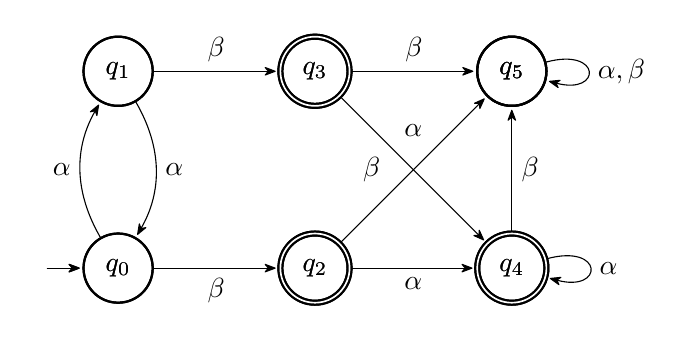
\begin{tikzpicture}[shorten >=1pt,node distance=2.5cm, on grid, >={Stealth[round]},initial text=,
        every state/.style={thick}]
        \node[state, initial] (q0) {$q_0$};
        \node[state, initial] (q0) {$q_0$};

        \node[state, above of=q0] (q1) {$q_1$};
        \node[state, above of=q0] (q1) {$q_1$};
        \node[state, accepting, right of=q0] (q2) {$q_2$};
        \node[state, accepting, right of=q0] (q2) {$q_2$};

        \node[state, accepting, above of=q2] (q3) {$q_3$};
        \node[state, accepting, above of=q2] (q3) {$q_3$};

        \node[state, accepting, right of=q2] (q4) {$q_4$};
        \node[state, accepting, right of=q2] (q4) {$q_4$};
        \node[state, right of=q3] (q5) {$q_5$};
        \node[state, right of=q3] (q5) {$q_5$};
        \node[state, right of=q3] (q5) {$q_5$};

        \path[->] (q0) edge[bend left] node[left]{$\alpha$} (q1);
        \path[->] (q0) edge node[below]{$\beta$} (q2);
        \path[->] (q1) edge[bend left] node[right]{$\alpha$} (q0);
        \path[->] (q1) edge node[above]{$\beta$} (q3);
        \path[->] (q2) edge node[below]{$\alpha$} (q4);
        \path[->] (q2) edge node[left=.3cm]{$\beta$} (q5);
        \path[->] (q3) edge node[above]{$\beta$} (q5);
        \path[->] (q3) edge node[above=.3cm]{$\alpha$} (q4);
        \path[->] (q4) edge[loop right] node[right]{$\alpha$} (q4);
        \path[->] (q4) edge node[right]{$\beta$} (q5);
        \path[->] (q5) edge[loop right] node[right]{$\alpha,\beta$} (q5);
    \end{tikzpicture}
    \caption{Note that $q_3$ has a transition to $q_4$ with an $\alpha$ and $q_2$ has a transition to $q_5$ with a $\beta$. There is no ambiguity since it is a DFA.}\label{ex1}
    \end{figure}

    \begin{table}[!ht]
        \centering
        \small
        \begin{tabular}{c|c|c}
            Splitter & Partition $\mathcal{P}$ & Workset $\mathcal{L}$\\
            \hline
            -- & $\{q_0,q_1, q_5\}\{q_2, q_3, q_4\}$ & $(\alpha, \{q_0,q_1, q_5\})\ (\beta, \{q_0,q_1, q_5\})$\\
            $(\beta, \{q_0,q_1, q_5\})$ & $\{q_0,q_1\}\{q_5\}\{q_2, q_3, q_4\}$ & $(\alpha, \{q_0,q_1\})\ (\alpha, \{q_5\})$\\
            $(\alpha, \{q_0,q_1\})$ & $\{q_0,q_1\}\{q_5\}\{q_2, q_3, q_4\}$ & $(\alpha, \{q_5\})$\\
            $(\alpha, \{q_5\})$ & $\{q_0,q_1\}\{q_5\}\{q_2, q_3, q_4\}$ & $\varnothing$\\
        \end{tabular}
    \end{table}
    Consider the automaton given in Fig. \ref{ex1}.
    Note that the partition is stable after the second iteration of the algorithm. The workset however changes after each iteration.
\end{remark}

Thus, it may happen that the estimate $\hat{T}$ does not decrease after a state transition where the partition does not change.
With the estimate $T$, we are sure that at each step, a splitter is used and thus a term in the sum over $\mathcal{L}$ is removed and ``goes'' into the sum over $\Sigma \times \mathcal{P} \setminus \mathcal{L}$\footnote{This remark is very informal.}.

However, because of the floor operation, we still cannot garantee that the estimate $T$ strictly decreases\footnote{Consider $\lfloor \log_2 n \rfloor$ and $\lfloor \log_2 n+1 \rfloor$: the bigger $n$ is, the more likely it is that both values are equal. Such terms might show up in border cases such as when a splitter splits off only one element from a block.}.
My thoughts on this are that ``most of the time'' there should exist at least one block in the partition that gets split in such a way that the corresponding term in the updated sum is strictly less than the term in the sum for the previous partition. The expression ``most of the time'' denotes a ``convenient split'', i.e.\ a split that actually cuts off a block in half or almost. In this case indeed, the term $\log n$ gets replaced by something close to $\log \frac{n}{2} = \log n - 1$.
However, in cases for example when a splitter splits off only one element from a block, the term $\log n$ gets replaced by $\log (n-1)$ which is not necessarily strictly less than $\log n$ (recall that $\log$ denotes $\lfloor \log_2 \rfloor$). Cases were such a split occurs for all blocks should be studied, if they exist. If no such cases exist, we would be provided with a good start of a proof that the estimate $T$ strictly decreases. Otherwise, we would have to examine classes of automaton individually and check that the estimate $T$ actually strictly decreases for each of them as well.

\section{Further work}
As mentioned above, finding a proof for a strict inequality is still a work in progress. It involves finding a suitable estimate, although the estimate $T$ seems to be a good candidate. However, this estimate makes the formalization more complex since it involves to consider separately elements from the workset and its complement and how they are affected by a state transition.

Everything linked to the estimate left aside, the formalization is still at a very early stage since we only focussed on the abstract level. However, this was the most important part of the formalization since it is the most complex one. The next steps would be to dive into the successive refinements and refine the abstract currencies. The formalization of the concrete currencies will be more straightforward since it will be mostly about implementing the abstract currencies with the chosen data structures, which probably already exists.

\section{Conclusion}

Although I was already quite used to working with Isabelle, this project was a great opportunity to improve my skills with the tool and in particular not to develop bad habits, since I had the best source of advice and help I could have hoped for: Peter Lammich, Tobias Nipkow and the whole team at his chair at TUM. I am very grateful for their help and I thank them heartfully for their time, patience and welcome.

Not only have I learned a lot about abstract concepts of formal verification, but I have also learned a lot about the implementation of Isabelle and its guts. I am now much more confident and my proofs -- be it for the \textit{apply}-style or the \textit{Isar}-style -- are much more robust and elegant. Even though intuition is not always a good feeling to follow in formal verification, mine has been strengthened as much as my creativity in terms of problem solving.

This project has given me a new taste of academic research and it has strengthened my will to pursue in this direction. Having been able to be part of such an internationally renowned team for a few months has been a great experience and I am very grateful for it.

% \printglossary[type=\acronymtype]

% \addcontentsline{toc}{section}{CV}
% \includepdf{cv.pdf}

\pagebreak
% bibliography
\bibliographystyle{alpha}
\bibliography{ref}

\end{document}